\chapter{Related Work} 
\label{cht:relatedwork}

We discuss related work in three related fields, XML fragmentation,
parallel XML processing and XML database Techniques.

\section{XML Fragmentation}

Fragmentation is a way of dividing an XML document into multiple smaller
fragments by physical changes so that these fragments can be allocated to
multiple computational nodes~\cite{BrMa14}. It is worth noting that the term
$fragment$ refers to a piece of XML document containing well-formed strucutre,
which allows us to perform faster or more efficient XML processing. It is
generally the premise of data-parallel computation algorithms. When process
large XML documents, it is a natural way to reduce the size of XML documents
processed at a time, so that we can process them with more computational nodes
in parallel to boost the perform of parsing and querying. For these reasons,
fragmentation has been intensively studied~\cite{ARBM06,DaGP14, CFKL12,NEMH07,
OgTP13,LiZZ17, CFKL12,DaGP14}. In this section, we discuss  two fragmentations
that closely relate to our study.


\subsection{Horizontal and Vertical Fragmentation}
\label{sec:hfragment}

There are two fragmentations defined by Kling et al.~\cite{kling11:dist_xml},
who modeled fragmentation as horizontal and vertical in terms of XML
schema~\cite{schema} that is a language for defnining the strucutre of XML
documents by constraints.

\subsubsection{Horizontal Fragmentation}
\label{sec:vfragment}

Horizontal fragmentation divides a document tree into multiple fragments and
each fragment follows the same schema as that of the original XML document. When
fragments follow the same schema, they usually have similar structure.  Let us
take the tree in Fig.~\ref{fig:hfrag_example} as an example. We divide the tree
into five subtrees, i.e. $d_1$, $d_2$,..., $d_5$ in the dotted rectangles.
According to the schema, a node `b' has a single `e' followed by one or zeor
`f'; a node `c' has exact one `e'; a node `d' can have zero or multiple node
`g's. Thus, all the subtrees follow the schema in
Fig.~\ref{fig:hfrag_example}(b). Note that all the root nodes of fragments are
at the same level, which is an intuitive reason why the fragmetation is called
horizontal fragmetation.


\begin{figure}[t]
	\centering
	\begin{subfigure}{.6\textwidth}
		\centering
		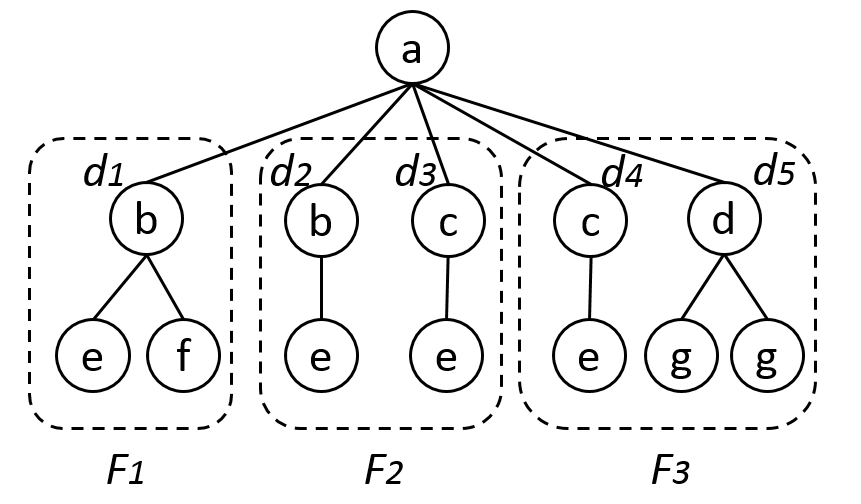
\includegraphics[width=.99\linewidth]{figures/hfrag_example}
		\caption{An example of horizontal fragmentation}
		\label{fig:sub1}
	\end{subfigure}%
	\begin{subfigure}{.4\textwidth}
		\centering
		\vspace{12mm}
		\begin{tabular}{|l|}
			\hline
			schema\\
			\hline
			a(b*, c*, d) \\
			b(e, f?) \\
			c(e) \\
			d(g*) \\
			\hline
		\end{tabular}
		\vspace{12mm}
		\caption{The schema of the example}
		\label{fig:sub2}
	\end{subfigure}
	\caption{An example of horizontal fragmentation and the schema.}
	\label{fig:hfrag_example}
\end{figure}

We then consider the whole document as a simple collection of fragments. Since
the fragments follow the same schema, the queries can be evaluated on them by
considering the schema. Horizontal fragmentation is rather straightforward and
thus widely used in parallel XML processing~\cite{DaGP14,BoLS09,AfDG15,CCMN15}.
In our study, we exploit and extend the horizontal fragmentation to process
large  XML document in distributed-memory environments.

\subsubsection{Vertical Fragmentation} 
\label{sec:vfragment}

Vertical fragmentation, on the other hand, is a fragmentation that also divides
an XML document into multiple fragments but at different levels, where these
fragments does not need to follow the same schemas. This fragmentation is
specially useful and works well for parallel XML processing in case XML data are
integrated from different sites or organizations~\cite{CFKL12,KlOD10}.


\subsection{Ad-hoc Fragmentation}

In comprison with horizontal and vertical fragmentation, ad-hoc fragmetation
does not consider the schema of XML documents. The partial tree (see Chapter 5)
in our study is a fragmetation that does not need the shcema of XML documents,
thus we consider this study can be categorized as ad-hoc fragmetation.

A common ad-hoc fragmentation is called /emph{hole-filler} model, where holes
are portals used for connection of fragments and fillers are fragments that can
connect to holes according to the structure of the original whole tree. Bose et
al. proposed a fragmentation model for steam data~\cite{bose2003query} and a
system called Xfrag~\cite{bose2005xfrag}. In their studies, an XML document is
divided into multiple sub documents, each of which has one or more holes  to
connect other sub document by the fillers that have some structrual information
to indicate the relationships to which a filler and a hole should be connected.
Another related work~\cite{lee2012memory}  proposed an improved hole-filler
model over streamed XML fragments, which is particularly designed for good 
memory-efficiency. Nomura et al. \cite{NEMH07} and Cong et al.~\cite{CFKL12}
adopted a tree-shaped fragment that contains original nodes and hole nodes,
where a hole node represents a link to a missing subtree, and represented the
whole document as a tree of fragments. Their approaches decouple dependencies
between evaluations on fragments so as to perform queries on them in parallel.



\section{Parallel XML Processing}
\label{sec:paralleleval}

Many existing studies address the topic of XML processing in
parallel~\cite{BoLS09,PaZC08,LuGa08,Mats09,SAFu05}. We discuss parallel XML
processing in this section.

\subsection{Tree Accumulation and Reduction}

There are some exsisting ideas of dividing the XML documents and running the
computation for trees called tree reduction. Kakehi et al.~\cite{KaME07} showed
a parallel tree reduction algorithm to the nodes in chunks. Based on the idea
given by Kakehi et al., Emoto and Imachi~\cite{EmIm12} developed a parallel tree
reduction algorithm on Hadoop, and Matsuzaki and Miyazaki~\cite{MaMi16}
developed a parallel tree accumulation algorithm. A similar approach was taken
by Sevilgen et al.~\cite{SAFu05} who developed a simpler version of tree
accumulations over the serialized representation of XML trees.

\subsection{XML Streaming}

Stream processing is a possible approach for (parallel) online data analysis.
Parallel algorithms have been studied to accelerate stream processing of large
XML data. For example, XMLTK~\cite{AGGR02} is an XML stream processing tool
designed for scalable XML querying. Y-Filter~\cite{ZhPC10} applies multiple
queries in parallel for a stream of XML data. Among these studies, Ogden et
al.~\cite{OgTP13} achieved the highest throughput, 2.5 GB/s, based on the
parallel pushdown transducer. Although it is the fastest oen and thus is faster
than our implementation of partial tree, which is 1 GB/s, the class of queries
we support is still more expressive than that of PP-transducer, which does not
support order-aware queries. In parallel pushdown transducers \cite{LiZZ17}, a
given document is modeled as a sequence of matched brackets and a fragment is
represented as a sequence of unmatched brackets.

\subsection{XML Parsing}

XML Parsing is a process of creating an XML tree from reading an XML document.
\cite{PLZC07,WZYu08} focused on XML parsing, which is related to our parsing
algorithm. Yinfei et al.~\cite{PaZC08} developed an algorithm for parsing the
XML data in parallel without any sequential preparsing phase.  Based on parallel
XML parsing, we propose partial tree that can achieve good load-balance by
dividing an XML document into many smaller fragments in similar sizes. A
similar idea was introduced by Choi et al.~\cite{ChLL14} in which they added
labels to construct a well-formed tree from a chunk in a preparsing phase. Compared to
fragmentation techniques on trees, the parallel XML parsing in  this study is
based on serialized text, which means we divide the plain text of an XML
document into multiple chunks in stead of fragmenting the  XML trees that are
parsed from the document.  The main advantage of our text-based fragmentation is
that we can easily achieve size-balance chunks and then process them over
distributed file systems~\cite{dfs}. 

\subsection{MapReduce-based XML Processing} \label{sec:mapreduce}

MapReduce~\cite{DeGh04} is a promising approach to large-scale XML processing,
which can run on top of clusters of commodity computers. It is suitalbe for
scalability as the size of XML data increases very rapidly.
Hadoop~\cite{HadoopWhit12}, which is a porpular implementtation of MapReduce, is
a common infrastructure for large-scale data processing, and to parallel
streaming~\cite{OgTP13,LiZZ17}. There have been several studies in this
direction~\cite{BCMU13,CFKL12,DaGP14,EmIm12,DaGP14,MaMi16}. One of earlier work
is by Choi et al.~\cite{CLKL12} called HadoopXML, which processes XML data in
parallel by applying SAX~\cite{sax} for each chunk. Including this work, most of
the existing MapReduce-based frameworks supports a small subset of XPath with
\texttt{child} and \texttt{descendant} axes with
predicates~\cite{CCMN15,AfDG15,DaGP14,DaGK14}. Instead, they extend the
expressiveness by the support of some query functionality (subsets of XQuery).
To cope with the problem of absolute performance of MapReduce, there is a few
work to use similar but more efficient frameworks, for example Apache
Flink~\cite{CCMN15}.

\subsection{Parallel Processing of queries}

Parallel XML processing has been actively studied after the paper presented by
Bordawekar et al.~\cite{BoLS09}, which closely relates to our study. The paper
proposes three strategies for XPath queries in parallel: data partition
strategy, query partition strategy, and hybrid partition strategy. . In fact,
there were some studies in the parallel programming community from 1990's.
Skillicorn developed a set of parallel computational patterns for trees called
tree skeletons, and showed they can be used for processing structured
documents~\cite{Skil97}. The main idea in parallelizing XPath queries was to
convert XPath queries into (tree) automata~\cite{comon2007tree}, and then
compute automata in parallel with tree skeletons. This idea was extended to
support a larger class of XPath including \texttt{following-sibling} by Nomura
et al.~\cite{NEMH07}. \cite{KrYa10,PLZC07,ZhPC10} focus on XPath queries
implemented in a shared-memory environment. \cite{AAHa11} proposed ideas about
XML processing in a forward and forward manner, which is helpful for our
research to support backward and upward queries as well. Liu et
al.~\cite{LFLQ08} developed a parallel version of structural join algorithm. The
study~\cite{ZaBS15} focuses processing a locality-aware partitioning in parallel
database systems. Cong et al.~\cite{CFKL12} formalized parallel processing of
XPath queries using the partial evaluation technique: the idea existing behind
their partial evaluation is similar to automata.

\section{XML Database Techniques}

\subsection{Indexing and Labeling Schemes}

Indexing is a commom database technique to improve the access of data  by using
index. It is also useful to for accelerating the access in XML databases.
However, due to the tree structure, it is a challenge to create efficient  index
for XML documents. In the early 2000, O'Neil et al.~\cite{OOPC04} proposed an
index called ORDPATH for natively supporting XML data type. This index makes it
possible to process XML queries inside the database with downward XPath queries
and allows update operations. Since this length of this index increases with
respect to the size of XML documents, the length will be very long in case the
XML documents are large. Pal et al.~\cite{PCSS04} studied how to improve the
query performance by introducing two indexes to nodes and values in SQL
Server~\cite{sql2005}. Li et al~\cite{LiLi05} improved OrdPath by reducing the
length of ORDPATH index when inserting. Min et al.~\cite{MLCh07} proposed an
efficient labeling scheme, called EXEL, which incurs no re-labeling of nodes
when inserting nodes. Finis et al~\cite{FBKF15} Proposed an idea mainly on how
to maintain and query hierarchical data at a high rate of complex, possibly
skewed structural updates. These indexes inspired our deisgn of index scheme on
XML document to make ours in a more efficient way. Besides these index schemes, 
there are also some studies concerning specific types of trees, such as
\cite{ToGr02,JLWO03,CVZZ08}, which examined the differences in indexing trees,
including B+-tree, R-tree, and XR-tree. In this theses, by considering the above 
studies, an new combined index is designed for representing partial tree to 
particularly process large XML data.

\subsubsection{Joins Algorithms}

Join processing is central to database implementation~\cite{graefe1993query}.
There are two join algorithms commonly used in XML processing, structural join
and twig join.

Structural join~\cite{AlJYK02} is mostly based on numbering
indexing\cite{numbering}, which numbers a nested intervals on nodes and is
commonly used in XML and other database
applications~\cite{ZNDI01,HAJR03,ZNDI01}. By using the information of start
position, end position and level of each node, the parent-child and
ancestor-descendant relationships of nodes can be determined by a merge join on
two lists of nodes. In 2001, a earily study~\cite{LiMo01} proposed three joint
algorithms for processing XML queries, which were similar to structural join. In
2002, Quanzhong Li et al. first proposed structural join in~\cite{AlJYK02}.
Jiang et al.~\cite{JLWO03} improved the structural join with a novel tree
structure, called XR-tree, which is suitable for identifying the descendants of
a given node with optimized worst case I/O cost. Le Liu et al.~\cite{LFLQ08}
first applied structural join in parallel over shared-memory environments.

Twig joins are also commonly used for maching a part of an XML
documents~\cite{jiang2003holistic,lu2005efficient,lu2005tjfast,
	fontoura2005optimizing}. In twig join, a query is represented as a twig patten,
and then is searched on the target XML document. One of the early twig joins was
\cite{BrKS02}. In the paper, a holistic twig join algorithm, called TwigStack
was proposed for matching an XML query. There are also variants of twig joins
then devleoped~\cite{CLTH06,QiYD07}. In 2009, Machdi et al.~\cite{MaAK09}
implemented the idea in parallel on multiple cores and in 2012 Choi et
al.~\cite{CLKL12} studied the twig joins on Hadoop in a parallel manner.
